\documentclass[conference]{IEEEtran}
%\IEEEoverridecommandlockouts
% The preceding line is only needed to identify funding in the first footnote. If that is unneeded, please comment it out.
\usepackage{cite}
\usepackage{amsmath,amssymb,amsfonts}
\usepackage{algorithmic}
\usepackage{graphicx}
\graphicspath{{images/}}
\usepackage{textcomp}
\usepackage{xcolor}
\usepackage{hyperref}

\def\BibTeX{{\rm B\kern-.05em{\sc i\kern-.025em b}\kern-.08em
    T\kern-.1667em\lower.7ex\hbox{E}\kern-.125emX}}
\begin{document}

\title{Does a higher quality of living contribute to a lower suicide rate?\\
}

\author{\IEEEauthorblockN{Owen Prosser}
\IEEEauthorblockA{\textit{School of Computer Science} \\
\textit{University of Lincoln}\\
Lincoln, United Kingdom \\
14514822@students.lincoln.ac.uk}
}

\maketitle

\begin{abstract}

\end{abstract}

\begin{IEEEkeywords}
developed, developing, suicide
\end{IEEEkeywords}

\section{Introduction}
Life is very diffent in any of the different countries on Earth. One's country of Birth or Country of residence
has a huge impact on all aspects of one's life. This paper investigates the existance of a link between
the standard of living of a country and it's rate of suicide.

\subsection{Motivation}
To discover if there is any link between Living Standards and Suicide rate which would be useful in aiding further
research into the other, more specific, causes. It has been shown that current state of the economy
has an impact on the suice rate when compared with historical data \cite{Suicides_2008-10}. This could result in more effective action being taken to combat this
issue and potentailly reduce the number suicides.

\subsection{Choice of Dataset}
The dataset for this paper was selected as it contained a wide set of detailed data on the subject.
It contains the data for around 117 countries from all over the globe and from all areas of the wealth and quality of living spectrum.
The dataset is also provided by a reliable source, the World Health Organisation (WHO).

\subsection{Research Hypothesis}
The Hypothesis for this paper was established by firstly analysing the dataset using descriptive statistics.
A total of six countries were selected for this paper with three on each end of the quality of living spectrum.
The top tree countries were selected based on the highest ``Social Progress Index’’ values of those countries contained within this dataset.
The ``Social Progress Index'' is based on three components, Basic Human Needs, Foundations of Wellbeing, and Opportunity\cite{high_standard_living}.
These are the Scandinavian countries, Sweden, Norway and the Netherlands.
The three lowest in the dataset are, Russia, Chile and Brazil.

The Histogram in Figure 1 shows that there is some correlation between the standard of living and the suiicde rate.
The two highest values of suicide per-capita are associated with two of the counties with the lowest standard of living.
This can justify further study into the hypothesis.

    \begin{figure}[hb]
        \centering
        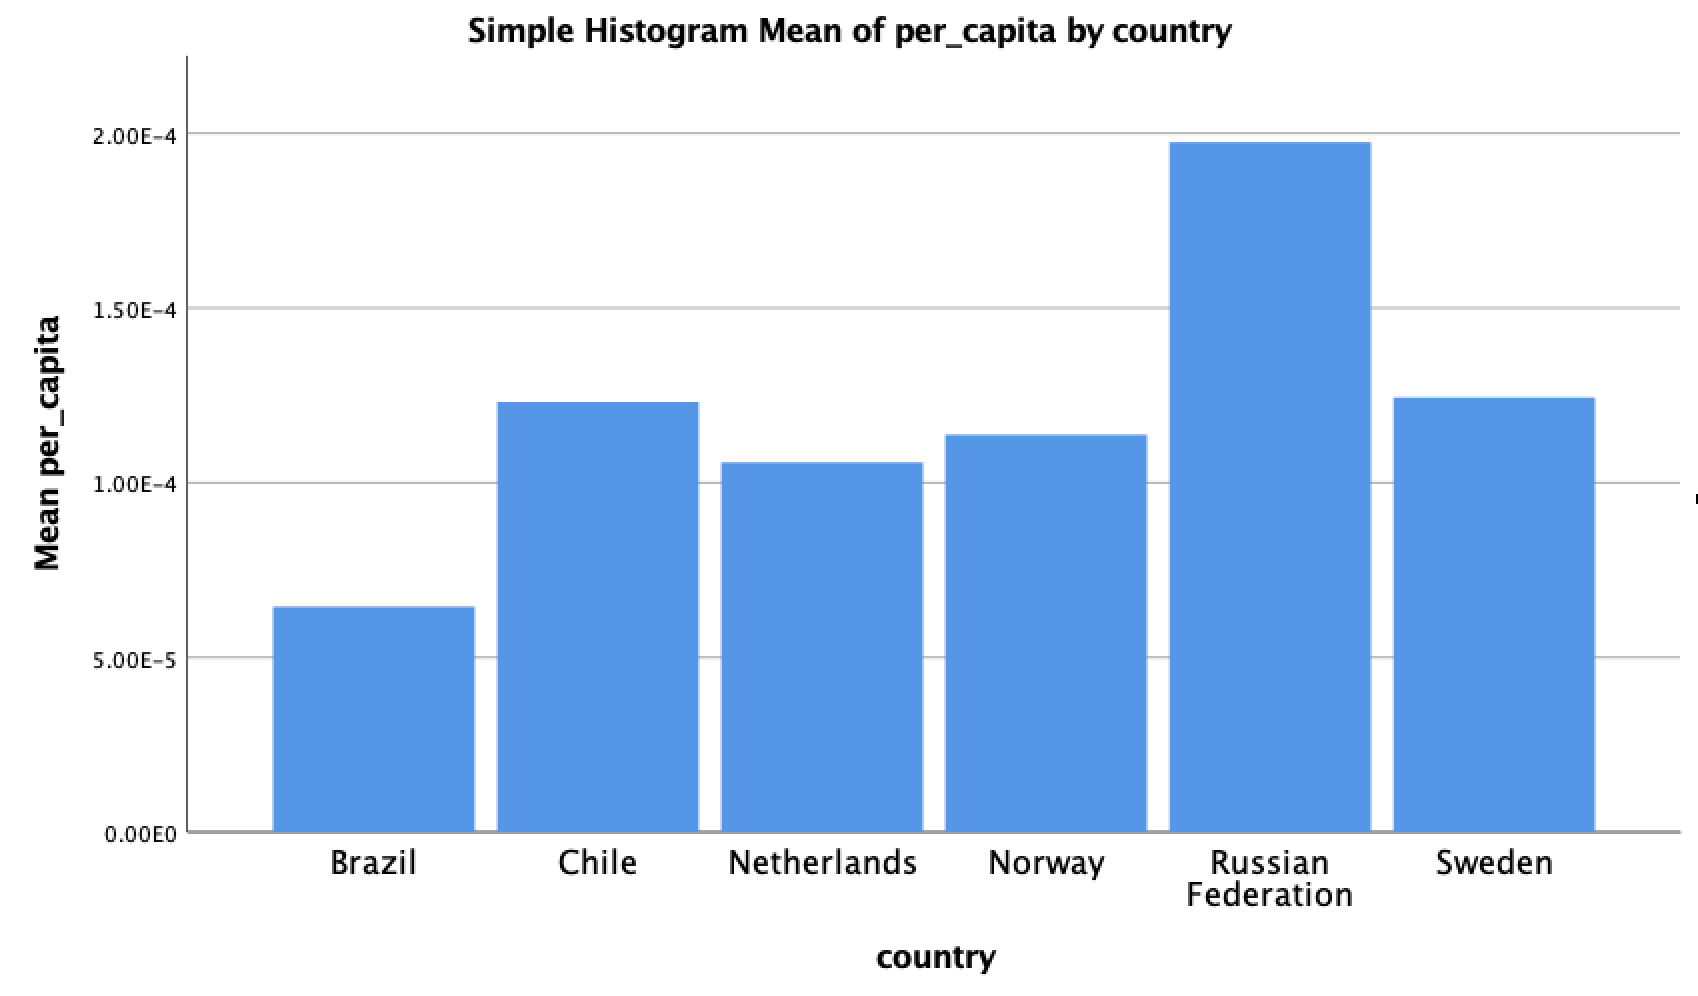
\includegraphics[width=0.4\textwidth]{percapita_bar}
        \caption{Histogram of the per-capita suicide rate of six countries.}
    \end{figure}

\section{Related Work}
``Suicide is the 15th leading cause of death worldwide, with over 75\% of suicides occurring in low-income and middle-income countries.''
Vijayakumar, Lakshmi, et al evaluated the links between the effects of the Human Development Index (HDI) and examined the
``association between a range of socioeconomic factors and suicide rate''.
In this case the studied countries were classified based on their HDI value in 2003 \cite{Sui_in_developing}.

\section{Methodology}

\section{Results}

\section{Conclusion}

\subsection{Future Work}

\begin{thebibliography}{00}
%\bibitem{b1} G. Eason, B. Noble, and I. N. Sneddon, ``On certain integrals of Lipschitz-Hankel type involving products of Bessel functions,'' Phil. Trans. Roy. Soc. London, vol. A247, pp. 529--551, April 1955.
\bibitem{Suicides_2008-10} Barr, B., Taylor-Robinson, D., Scott-Samuel, A., McKee, M. and Stuckler, D., "Suicides associated with the 2008-10 economic recession in England: time trend analysis". Bmj, 345, p.e5142, 2012..
\bibitem{high_standard_living} M. Smith, ``The 19 countries with the highest standard of life'', Business Insider. New York, 2016.
\bibitem{Sui_in_developing}Vijayakumar, Lakshmi, et al. "Suicide in Developing Countries (1) Frequency, Distribution, and Association with Socioeconomic Indicators." Crisis 26.3 (2005): 104-111
\end{thebibliography}
\vspace{12pt}

\end{document}
